\documentclass[12pt]{beamer}
\usetheme{CambridgeUS}
\usepackage[utf8]{inputenc}
\usepackage[german]{babel}
\usepackage[T1]{fontenc}
\usepackage{amsmath}
\usepackage{amsfonts}
\usepackage{amssymb}
\usepackage{graphicx}
\author{Florian Kluibenschedl}
\title{Direkte Analyse von Chlorophyllkataboliten}
%\setbeamercovered{transparent} 
%\setbeamertemplate{navigation symbols}{} 
%\logo{} 
%\institute{} 
%\date{} 
%\subject{} 
\begin{document}

\begin{frame}
\titlepage
\end{frame}

%\begin{frame}
%\tableofcontents
%\end{frame}

\begin{frame}{Zielsetzung}
 \begin{itemize}
 \item Analyse der Chl-Kataboliten des Brokkoli Blattes
 \item Modifikation durch Reaktion
 \end{itemize}
\end{frame}

\begin{frame}{Ergebnisse}
 \begin{itemize}
 \item 6 Chl-Kataboliten identifiziert
 \item Strukturvorschläge konnten gemacht werden
 \item MS-Leafspray eignete sich als Methode
 \item Reaktionsprodukte durch Massenzunahme nachgewiesen
 \end{itemize}
\end{frame}

\begin{frame}{Das Modell und Fragmentierungsdiagramme - der spannende Teil ;)}
 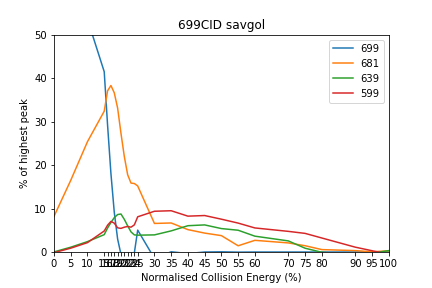
\includegraphics[scale=0.65]{699CID-savgol1.png}
\end{frame}

\begin{frame}{Vielen Dank für Ihre Aufmerksamkeit}
P.S.:
 \begin{itemize}
 \item Chl-Kataboliten sind (vermutlich) gute Antioxidantien
 \item Brokkoli avancierte zu meiner Lieblingsfrucht
 \end{itemize}
\end{frame}

\end{document}